% Created 2018-10-28 søn 15:17
% Intended LaTeX compiler: pdflatex
\documentclass[12pt]{article}

%%%% settings when exporting code %%%% 

\usepackage{listings}
\lstset{
backgroundcolor=\color{white},
basewidth={0.5em,0.4em},
basicstyle=\ttfamily\small,
breakatwhitespace=false,
breaklines=true,
columns=fullflexible,
commentstyle=\color[rgb]{0.5,0,0.5},
frame=single,
keepspaces=true,
keywordstyle=\color{black},
literate={~}{$\sim$}{1},
numbers=left,
numbersep=10pt,
numberstyle=\ttfamily\tiny\color{gray},
showspaces=false,
showstringspaces=false,
stepnumber=1,
stringstyle=\color[rgb]{0,.5,0},
tabsize=4,
xleftmargin=.23in,
emph={anova,apply,class,coef,colnames,colNames,colSums,dim,dcast,for,ggplot,head,if,ifelse,is.na,lapply,list.files,library,logLik,melt,plot,require,rowSums,sapply,setcolorder,setkey,str,summary,tapply},
emphstyle=\color{blue}
}

%%%% packages %%%%%

\usepackage[utf8]{inputenc}
\usepackage[T1]{fontenc}
\usepackage{lmodern}
\usepackage{textcomp}
\usepackage{color}
\usepackage{enumerate}
\usepackage{graphicx}
\usepackage{grffile}
\usepackage{wrapfig}
\usepackage{rotating}
\usepackage{longtable}
\usepackage{multirow}
\usepackage{multicol}
\usepackage{changes}
\usepackage{pdflscape}
\usepackage{geometry}
\usepackage[normalem]{ulem}
\usepackage{amssymb}
\usepackage{amsmath}
\usepackage{amsfonts}
\usepackage{dsfont}
\usepackage{textcomp}
\usepackage{array}
\usepackage{ifthen}
\usepackage{hyperref}
\usepackage{natbib}
\pagestyle{empty} % no page numbering
\usepackage[french, frenchb]{babel}
\newcommand{\Rlogo}{\textbf{\textsf{R}}}
\newcommand{\Cpp}{C\nolinebreak\hspace{-.05em}\raisebox{.4ex}{\tiny\bf +}\nolinebreak\hspace{-.10em}\raisebox{.4ex}{\tiny\bf +}}
\usepackage{eurosym} % euro symbol
\usepackage{titlesec}
\titleformat{\section}{\large}{\thesection}{1em}{}
\titlespacing*{\section}{0pt}{0.25\baselineskip}{0.25\baselineskip}
\geometry{
left=20mm,
right=20mm,
top=20mm,
bottom=20mm
}
\RequirePackage{setspace} % to modify the space between lines - incompatible with footnote in beamer
\renewcommand{\baselinestretch}{1.1}
\usepackage{framed}
\usepackage{tocloft}
\newlength{\outerbordwidth}
\raggedbottom
\raggedright
\setlength{\outerbordwidth}{3pt}  % Width of border outside of title bars
\definecolor{shadecolor}{gray}{0.75}  % Outer background color of title bars (0 = black, 1 = white)
\definecolor{shadecolorB}{gray}{0.93}  % Inner background color of title bars
\usepackage{mdframed}
\newcommand{\resitem}[1]{\item #1 \vspace{-2pt}}
\newcommand{\resheading}[1]{
\vspace{8pt}
\parbox{\textwidth}{\setlength{\FrameSep}{\outerbordwidth}
\begin{shaded}
\setlength{\fboxsep}{0pt}\framebox[\textwidth][l]{\setlength{\fboxsep}{4pt}\fcolorbox{shadecolorB}{shadecolorB}{\textbf{\sffamily{\mbox{~}\makebox[6.762in][l]{\large #1} \vphantom{p\^{E}}}}}}
\end{shaded}
}\vspace{-5pt}
}
\newcommand{\ressubheading}[4]{
\begin{tabular*}{6.5in}{l@{\cftdotfill{\cftsecdotsep}\extracolsep{\fill}}r}
\textbf{#1} & #2 \\
\textit{#3} & \textit{#4} \\
\end{tabular*}\vspace{-6pt}}
\usepackage{bibentry}
\nobibliography*
\newcommand{\myname}[1]{\textbf{#1}}
\usepackage{url}
\date{\today}
\title{}
\hypersetup{
 colorlinks=true,
 citecolor=[rgb]{0,0.5,0},
 urlcolor=[rgb]{0,0,0.5},
 linkcolor=[rgb]{0,0,0.5},
 pdfauthor={Brice Ozenne},
 pdftitle={},
 pdfkeywords={},
 pdfsubject={},
 pdfcreator={Emacs 27.0.50 (Org mode 9.0.4)},
 pdflang={Frenchb}
 }
\begin{document}

\begin{tabular*}{7in}{l@{\extracolsep{\fill}}r}
	\textbf{\Large Brice Ozenne} & \textbf{\today} \\
\end{tabular*}

\vfill

\begin{minipage}{0.2\linewidth}
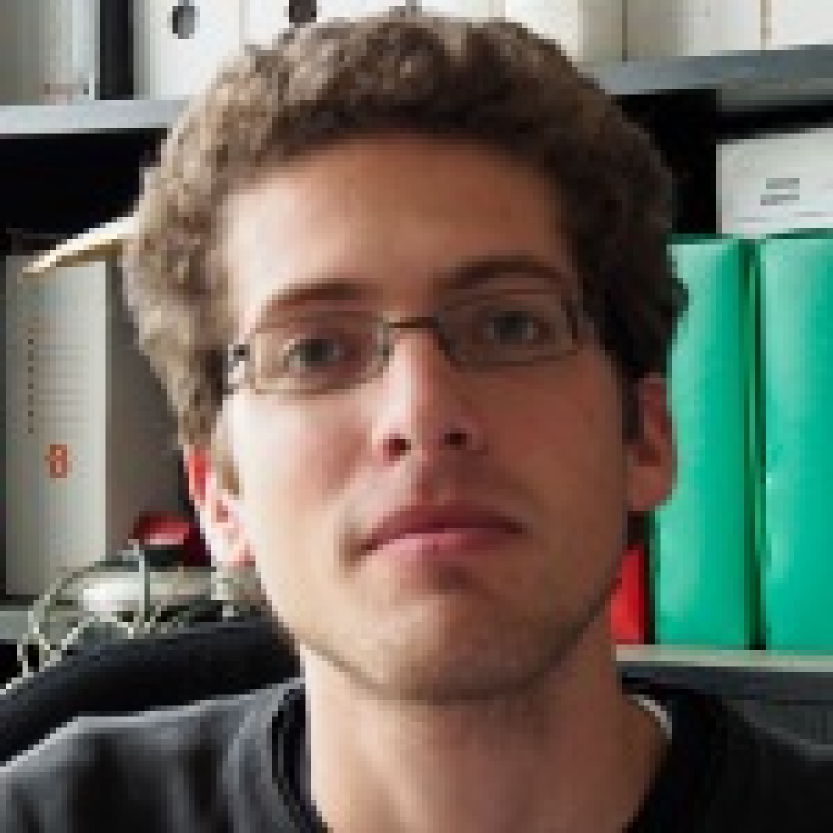
\includegraphics[width=\linewidth]{photoId.png}
\end{minipage}
\begin{minipage}{0.75\linewidth}
\begin{tabular*}{7in}{ll@{ }l}
	Nationalité&:& français  \\
	Né&:& le 8 février 1990 à Saint Hilaire du Harcouët (50)  \\
	Courriel personnel&:& \url{brice.ozenne@orange.fr} \\ 
	Téléphone personnel&:& (+45) 52 328 128 \\ 
        Adresse personnelle&:& 3 Emblasgade, 1 t.h., 2100 Copenhagen Ø, Danemark \\
\end{tabular*}
\end{minipage}

\vfill

\resheading{Activité de recherche}
\begin{tabular}{l@{ }l}
	Novembre 2015- Actuellement:& \textbf{Post doctorant} (\href{http://publichealth.ku.dk/staff/?pure=en/persons/540231}{page personnelle})\\
	& Section of Biostatistics, University of Copenhagen \\
	& Øster Farimagsgade 5, 1014 Copenhague, Danemark \\
	& \\
	& Neurobiology Research Unit \\
	& Copenhagen University Hospital, Rigshospitalet \\
	& Building 6931, Blegdamsvej 9, DK-2100 Copenhagen, Denmark
\end{tabular}

\bigskip

Mon travail de recherche s'articule autour de trois thèmes:
\begin{itemize}
\item le développement de \textbf{modèles à variables latentes} pour l'analyse de
données complexes (logiciel \texttt{lavaSearch2}). Ces travaux trouvent leur application dans
l'analyse des données issues de neuroimagerie ou de tests
psychologiques.
\end{itemize}

\smallskip

\begin{itemize}
\item l'analyse de données de \textbf{survie en présence de risques compétitifs}
sur données de registres (logiciel \texttt{riskRegression}). Ces méthodes sont utilisées pour comparer
l'efficacité de traitements préventifs de maladies cardiovasculaires
à l'aide des données des registres danois.
\end{itemize}

\smallskip

\begin{itemize}
\item l'extension des \textbf{méthodes de comparaison par paires},
permettant d'évaluer la balance bénéfice-risque d'un traitement avec
des critères de jugement de différentes natures (logiciel \texttt{BuyseTest}). Plusieurs
applications de cette méthode ont été publiées lors de l'évaluation
de chimiothérapies.
\end{itemize}

\vfill

\resheading{Formation Universitaire}
\begin{tabular}{l@{ }l}
2012 - 2015 : & Doctorat en biostatistiques, Université Lyon 1. \\
\multicolumn{2}{l}{Sujet: \href{https://tel.archives-ouvertes.fr/tel-01233049/document}{Modélisation statistique pour le pronostic de patients atteints d’un Accident Vasculaire Cérébral}} \\ [3mm]
2009 - 2012 : &  École Centrale de Lyon, formation d'ingénieur généraliste avec spécialisation en statistiques \\ 
              & Erasmus à l'université Politecnico di Milano (2nd semestre 2011) \\
              & Master en biostatistiques à l'Université Lyon 1 en double diplôme (\href{http://mastersantepublique.univ-lyon1.fr/webapp/website/website.html?id=3124911&pageId=215838}{M2 B3S}). \\
\end{tabular}

\vfill

\clearpage

\resheading{Compétences}
\section*{\emph{Linguistiques}}
\label{sec:org46770e2}
Français (langue maternelle), anglais (courant), notions d'italien et de danois.

\section*{\emph{Logicielles}}
\label{sec:org2e83dca}
Bonne connaissance de \Rlogo{}, \LaTeX{} et \href{https://orgmode.org/}{orgmode}. \\
Utilisation courante mais basique de \Cpp{}, lisp (pour \href{https://www.gnu.org/software/emacs/}{GNU Emacs}) et
git/github (via \href{https://magit.vc/}{magit}).
\resheading{Financement}
\begin{tabular}{l@{ }l}
2017-2019: MARIE CURIE Individual Fellowships (200 000\euro) \\
2017-2020: Lundbeck Fellowships (140 000\euro) \\

\end{tabular}


\resheading{Production scientifique}
\section*{\emph{Publications (méthodologiques)}}
\label{sec:org8085cb4}

Publié:
\begin{enumerate}
   \item \bibentry{ozenne2017riskregression}
   \item \bibentry{peron2016extension}
   \item \bibentry{ozenne2015precision}
   \item \bibentry{ozenne2015spatially}
 \end{enumerate}
Soumis:
\begin{enumerate}
   \item \bibentry{ozenne20XXestimation}
   \item \bibentry{ozenne20XXsmall}
 \end{enumerate}
En cours de rédaction:
\begin{enumerate}
   \item \bibentry{ozenne20XXcontroling}
   \item \bibentry{peron20XXunbiased}
 \end{enumerate}

\section*{\emph{Développement logiciel (librairies pour le logiciel \href{https://www.r-project.org/}{R})}}
\label{sec:org8d89057}
\begin{minipage}{0.01\textwidth}
\hspace{\fill}
\end{minipage}
\begin{minipage}{0.92\textwidth}
\begin{itemize}
\item \textbf{BuyseTest} (Créateur et mainteneur) : Comparisons par paires
généralisées. Implémentation de la méthode décrite dans
\citep{peron2016extension}. Disponible sur le \href{https://cran.r-project.org/web/packages/BuyseTest/index.html}{CRAN} et sur \href{https://github.com/bozenne/BuyseTest}{Github}.

\item \textbf{lavaSearch2} (Créateur et mainteneur) : Inférence et outils
diagnostiques dans les modèles à variables latentes. Papier
décrivant la méthode soumis. Disponible sur le \href{https://cran.r-project.org/web/packages/lavaSearch2/index.html}{CRAN} et sur \href{https://github.com/bozenne/lavaSearch2}{Github}. .

\item \textbf{riskRegression} (Contributeur) : Calculateur du risque
d'évènenement en présence de risques compétitifs. Implémentation de
la méthode décrite dans \citep{ozenne2017riskregression}. Disponible
sur le \href{https://cran.r-project.org/web/packages/riskRegression/index.html}{CRAN} et sur \href{https://github.com/tagteam/riskRegression}{Github}.
\end{itemize}
\end{minipage}

\bigskip

\section*{\emph{Publications (applications cliniques)}}
\label{sec:org70821b6}
\begin{enumerate}
   \item \bibentry{borgsted2018amygdala}
   \item \bibentry{hjordt2018self}
   \item \bibentry{foged2018verbal}
   \item \bibentry{staerk2018standard}
   \item \bibentry{hjordt2017season}
   \item \bibentry{beliveau2017high}
   \item \bibentry{stenbaek2017brain}
   \item \bibentry{staerk2017resumption}
   \item \bibentry{fisher2017bdnf}
   \item \bibentry{foged2017safety}
   \item \bibentry{peron2016net}
   \item \bibentry{staerk2016ischaemic}
   \item \bibentry{peron2016assessment}
   \item \bibentry{ozenne2015evaluation}
   \item \bibentry{hermitte2013very}
 \end{enumerate}
\resheading{Enseignement \hfill CM : cours magistral, TD : travaux dirigés}
\begin{tabular}{l@{ }l}
2016 - 2017 : & \href{http://publicifsv.sund.ku.dk/~jufo/RepeatedMeasures2016.html}{Analyse statistique de données répétées}. TD pour doctorants en médecine (18h). \\
              & \href{http://publicifsv.sund.ku.dk/~kkho/undervisning/sem2016/}{Modèles d'équations structurelles}. CM pour étudiants de master en statistiques (2h) \\
2015 - 2016 : & \href{http://publicifsv.sund.ku.dk/~jufo/RepeatedMeasuresE2015.html}{Analyse statistique de données répétées}. TD pour doctorants en médecine (18h). \\
2014 - 2015 : & \href{http://mastersantepublique.univ-lyon1.fr/webapp/website/website.html?id=3124911&pageId=215839}{Modèles de Survie}. TD pour étudiants de master en santé publique (18h).\\
              & \href{http://mastersantepublique.univ-lyon1.fr/webapp/website/website.html?id=3124911&pageId=215839}{Statistique bayésienne}. TD pour étudiants de master en santé publique (18h).\\
2013 - 2014 : & \href{http://mastersantepublique.univ-lyon1.fr/webapp/website/website.html?id=3124911&pageId=215839}{Statistique bayésienne}. TD pour étudiants de master en santé publique (6h).\\
\end{tabular}

\resheading{Encadrement}
\begin{tabular}{l@{ }l@{ }l}
2015 - Actuellement &:& \textbf{consultant} en statistiques pour NRU (\href{https://nru.dk/}{Neurobiology Research Unit}).  \\ 
\multicolumn{3}{l}{ Conseille les chercheurs en neuroscience dans l'analyse de leurs données et la rédaction d'articles.} \\ [3mm]
                        2014 &:& encadrement d'une étudiante de master 2 dans son stage de fin d'étude. \\
\end{tabular}


\bibliographystyle{plainnat}

\nobibliography{publicationBO}
\end{document}